\begin{preface}
    “The test of successful education is not the amount of knowledge that pupils take away from school, but their appetite to know and their capacity to learn.” 
    -Sir Richard Livingstone 1941. \cite{Livingstone}
    
    La ricerca moderna, conseguentemente al fenomeno della pandemia da Covid-19, ha riservato attenzione sempre maggiore al tema della fruizione di contenuti, sia dal punto di vista dell’intrattenimento che dal punto di vista della produttività individuale.
    
    La pandemia ha quindi consentito alla ricerca l’impiego di strumenti impattanti in questo campo, in quanto ormai possibile osservare e quindi analizzare, le attitudini comportamentali del singolo, per migliorare l’esperienza di utilizzo dei prodotti software.
    
    Effettuando diverse ricerche a riguardo ho potuto constatare che la maggior parte degli studi precedentemente effettuati si concentra sull’analisi delle emozioni che vengono categorizzate come primarie dal sistema FACS (Facial Action Coding System) \cite{FacialCodingContinMonitor}:
    \begin{itemize}
        \item Happiness,
        \item Anger,
        \item Sadness,
        \item Disgust,
        \item Fear,
        \item Neutral
    \end{itemize}
    
    Di contro argomenti quali gli stati d’animo (o mood), che influenzano l’engagement degli studenti durante l’apprendimento, sono stati ampiamente trascurati.
    
    Diversi studi hanno dimostrato che gli stati d’animo positivi sono direttamente collegati al pensiero creativo e alla capacità dell’individuo di riflettere su ciò che sta compiendo, indi una maggiore agevolezza e beneficio nell’apprendimento che ne consegue; diversamente gli stati d’animo negativi sono correlati ad una maggiore difficoltà di esercitare queste caratteristiche portando ad un minore rendimento relativamente a questo ambito.
    
    Per quanto le emozioni primarie forniscano sicuramente un indicatore dello stato d’animo, e del conseguente miglioramento dell’esperienza di apprendimento o di lavoro, non sono però generalmente manifestate in modo esplicito, soprattutto per quanto concerne le espressioni facciali, in contesti di ufficio e studio.
    
    Coerentemente si è ritenuto fondamentale concentrare lo studio sulle espressioni facciali e i mood più frequenti all’interno di questi ambienti.
    
    Nei prossimi paragrafi analizzerò degli studi riguardanti sia l’analisi degli stati d’animo e i relativi procedimenti adoperati per effettuarli, che uno studio inerente alle FACS, dove vengono analizzati vari algoritmi, successivamente posti a confronto, per la costruzione di un modello basato sui dati estratti dalle relative immagini.
    
    \begin{figure}
        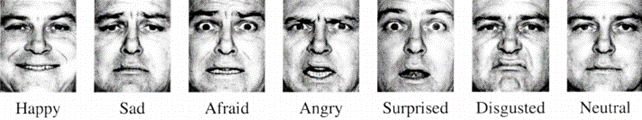
\includegraphics[width=1\linewidth]{images/1.png}
        \caption{Emozioni nel sistema FACS}
    \end{figure}
\end{preface}